\documentclass{beamer}

\usetheme{Luebeck}
\usefonttheme{serif}
\usecolortheme{seagull}
\usepackage{graphicx}
\DeclareGraphicsExtensions{.pdf,.png,.jpg}

\usepackage{epsfig}
\usepackage{tikz}
\usetikzlibrary{arrows}
\tikzstyle{block}=[draw opacity=0.7,line width=1cm]

\title[Spike Train Analysis]
{
Spike Train Analysis: \\ Estimating the firing rate of a simple \\model neuron from its spike train
}

\author{
Cathal Cooney
}

\institute[TCD]
{
School of Maths, Trinity College Dublin
}

\date{2nd April 2015}

\begin{document}

\begin{frame}
\titlepage
\end{frame}

\begin{frame}
\frametitle{Overview}
\tableofcontents
\end{frame}

\section{Introduction}
\subsection{Computational Neuroscience}
\begin{frame}
\frametitle{Introduction to Computational Neuroscience}
\begin{itemize}
\item Neural data is highly temporal, and data sets can be very large.
\pause
\bigskip
\item Computers are therefore widely used to aid the analysis of neural data.
\pause
\bigskip
\item Mathematicians, physicists and engineers have looked to use their skills to analyse data and model phenomena.
\end{itemize}
\end{frame}

\subsection{Spike Trains}
\begin{frame}
\frametitle{Spikes}
\begin{itemize}
\item Spikes are the electrical signals that propagate through the brain. 
\pause
\bigskip
\item They consist of a rapid depolarisation and subsequent hyper-polarisation of the membrane potential.
\pause
\bigskip
\item A neuron either spikes or it doesn't, there are no fractional spikes.
\pause
\bigskip
\item A neuron's spikes tend to have a typical voltage profile.
\end{itemize}
\end{frame}

\begin{frame}
\frametitle{Example spike}
\begin{center}
\begin{figure}
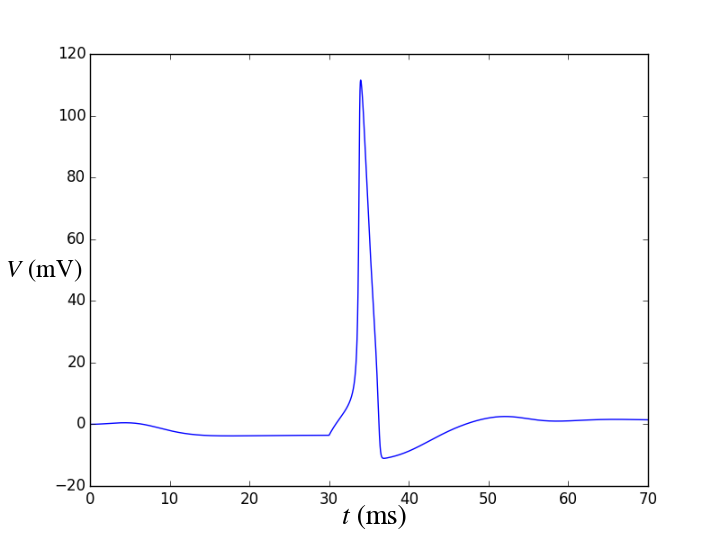
\includegraphics[width=0.75\textwidth]{hh.png}
\end{figure}
\end{center}
\end{frame}

\begin{frame}
\frametitle{Spike Trains}
\begin{itemize}
\item Spike trains can be described by just their times. \pause \\ \bigskip
\item So, if a neuron has $n$ spikes at times $t_i$, $i=1,\ldots,n$.\pause
\end{itemize}
\begin{equation*}
X = x(t) = \sum_{i=1}^{n} \delta \left( t - t_i \right)
\end{equation*}
\pause
\bigskip

Spike trains are typically treated as point processes in computational neuroscience.
\end{frame}

\section{Neuron Model}
\subsection{Definition}
\begin{frame}
\frametitle{Motivation and assumptions}
\begin{itemize}
\item It has been observed that some neurons spike at a much higher rate when specific features are present in the stimuli. \pause \\(eg. grandmother/Jennifer Aniston neuron)
\pause
\bigskip
\item A simple neuron model is proposed, where a \lq{}neuron\rq{} is said to either be in an \lq{}up-state\rq{} or an \lq{}down-state\rq{}.
\pause
\bigskip
\item It is assumed that the features are very specific, so most neurons would be \lq{}down\rq{} more than they are \lq{}up\rq{}.
\pause
\bigskip
\item This is typical of \emph{sparse coding}, which has been shown to be an energy-efficient coding scheme in the brain.
\end{itemize}
\end{frame}

\begin{frame}
\frametitle{The Model}
\begin{center}
\setlength{\unitlength}{.055cm}
\begin{picture}(150,75)
\put(0,14){\mbox{$\lambda_d$}}
\put(0,34){\mbox{\small{$\lambda_u$}}}

\linethickness{1.5pt}
\put(7,10){\line(1,0){138}}
\put(7,55){\line(1,0){138}}

\linethickness{1pt}
\put(7,15){\line(1,0){18}}
\put(15,15){\vector(0,1){8}}
\put(17,17){\mbox{$u$}}
\put(25,15){\line(0,1){20}}
\put(25,35){\line(1,0){30}}
\put(38,35){\vector(0,-1){8}}
\put(40,29){\mbox{$d$}}
\put(55,35){\line(0,-1){20}}
\put(55,15){\line(1,0){40}}
\put(73,15){\vector(0,1){8}}
\put(75,17){\mbox{$u$}}
\put(95,15){\line(0,1){20}}
\put(95,35){\line(1,0){25}}
\put(106,35){\vector(0,-1){8}}
\put(108,29){\mbox{$d$}}
\put(120,35){\line(0,-1){20}}
\put(120,15){\line(1,0){25}}
\put(132,15){\vector(0,1){8}}
\put(134,17){\mbox{$u$}}

\put(27,55){\line(0,1){15}}
\put(35,55){\line(0,1){15}}
\put(46,55){\line(0,1){15}}
\put(50,55){\line(0,1){15}}

\put(67,55){\line(0,1){15}}
\put(84,55){\line(0,1){15}}

\put(100,55){\line(0,1){15}}
\put(107,55){\line(0,1){15}}
\put(116,55){\line(0,1){15}}
\put(135,55){\line(0,1){15}}

\multiput(8,35)(5,0){28}{\line(1,0){2}}
%\multiput(8,15)(5,0){28}{\line(1,0){2}}
\end{picture}
\bigskip \\
The model assumes that the neuron is a bimodal Poisson process, with constant firing rates $\lambda_u$ and $\lambda_d$. \pause The \lq{}switching rates\rq{}, $u$ and $d$, are also assumed to be constant Poisson rates.
\end{center}
\end{frame}

\subsection{Markov Chains}
\begin{frame}
\frametitle{Markov Chains}
\begin{itemize}
\item The on/off - states form a \emph{Markov chain}; there is no extra information to be gained by knowing the history of the process.
\end{itemize}
\begin{equation*}
P\left( x(t_0+h)=A \,| x(t), t \leq t_0 \right) = P \left( x(t_0+h)=A \,| x(t_0)\right)
\end{equation*}
\pause

For the up/down-states, the Markov chain is described as:
\begin{equation*}
P^\prime (t)= P(t)Q, \mbox{ where } Q = \begin{pmatrix} -d & d \\ u & -u \end{pmatrix}
\end{equation*}
\end{frame}

\begin{frame}
\frametitle{Markov Chains}
So, if the probability, $p_u(t_0)$, of being in the up-state is known at a time $t_0$, then:
\begin{equation*}
P(t) = P(t_0)e^{(t-t_0)Q}
\end{equation*}
and 
\begin{equation*}
 p_u(t) = \frac{u}{u+d}\left( 1 - e^{-(u+d)(t-t_0)}\right) + p_u(t_0)e^{-(u+d)(t-t_0)}
\end{equation*}
\pause

However, this ignores the differing spiking rates of the two states.
\end{frame}

\begin{frame}
\frametitle{Absorption State}
\begin{itemize}
\item By restricting the viewpoint to between any two spikes, a new Markov chain is formed.
\pause
\item The state of spiking is introduced as an \lq{}absorption state\rq{} to the previous Markov chain.
\pause
\item That is, there is no return possible to the up/down - states having spiked.
\end{itemize}
\pause
This has transition matrix $Q_s$:
\begin{equation*}
Q_s = \begin{pmatrix} -d-\lambda_u & d & \lambda_u \\ u & -u-\lambda_d & \lambda_d \\ 0 & 0 & 0 \end{pmatrix}
\end{equation*}
\end{frame}

\begin{frame}
\begin{center}
\setlength{\unitlength}{.07cm}
\begin{picture}(120,75)
\put(90,37){\mbox{$\lambda_d$}}
\put(25,37){\mbox{$\lambda_u$}}
\put(59,67){\mbox{$d$}}
\put(59,49){\mbox{$u$}}

\put(25,60){\oval(40,25)}
\put(21,58){\mbox{{\bf UP}}}
\put(95,60){\oval(40,25)}
\put(85,58){\mbox{{\bf DOWN}}}
\put(60,20){\oval(40,25)}
\put(51,18){\mbox{{\bf SPIKE}}}

\put(45,65){\vector(1,0){30}}
\put(75,55){\vector(-1,0){30}}
\put(25,47.5){\vector(4,-3){21}}
\put(95,47.5){\vector(-4,-3){21}}
\end{picture}
\end{center}
\pause
Between any two spikes, this Markov chain determines the probability of being in the up-state or the down-state. By setting $t_0=0$, this has solution:
\begin{equation*}
P(t) = P(0)e^{tQ_s}
\end{equation*}
\end{frame}

\subsection{Firing Rate}
\begin{frame}
\frametitle{Estimated Firing Rate}
Then the firing rate is calculated as:
\begin{equation*}
r(t) = \lambda_u p_u(t) + \lambda_d\left(1-p_u(t)\right) = (\lambda_u - \lambda_d)p_u(t) + \lambda_d
\end{equation*}
\pause
\bigskip
If the firing rate at $t=0$ is $r_0$, then this has the very nice form:
\begin{equation}
r(t) = \frac{\alpha\left( \beta - r_0 \right) e^{-\alpha t} + \beta\left( r_0 - \alpha\right)e^{-\beta t}}{\left( \beta - r_0 \right) e^{-\alpha t} + \left( r_0 - \alpha\right)e^{-\beta t}}
\end{equation}
where $-\alpha,-\beta$ are the non-zero eigenvalues of $Q_s$.
\end{frame}

\begin{frame}
\frametitle{What about spikes?}
\pause
\begin{itemize}
\item The firing rate is now known between any two spikes, provided it can be re-calculated at the arrival of each spike.
\pause
\item Use Bayes' theorem to calculate the change at the arrival of each spike.
\end{itemize}
\begin{equation*}
\begin{split}
P(\mbox{up-state} | \mbox{spike}) &= \frac{P(\mbox{spike}|\mbox{up-state})P(\mbox{up-state})}{P(\mbox{spike})} \\
&=\frac{\lambda_u p_u(t)}{(\lambda_u - \lambda_d) p_u(t) + \lambda_d }
\end{split}
\end{equation*}
\pause
In term of the firing rate, get:
\begin{equation}
r(t) \mapsto (\lambda_u + \lambda_d) - \frac{\lambda_u\lambda_d}{r(t)}
\end{equation}
\end{frame}

\begin{frame}
\frametitle{Firing Rate Estimate}
\begin{center}
\resizebox{0.8\textwidth}{!}{% GNUPLOT: LaTeX picture with Postscript
\begingroup
  \makeatletter
  \providecommand\color[2][]{%
    \GenericError{(gnuplot) \space\space\space\@spaces}{%
      Package color not loaded in conjunction with
      terminal option `colourtext'%
    }{See the gnuplot documentation for explanation.%
    }{Either use 'blacktext' in gnuplot or load the package
      color.sty in LaTeX.}%
    \renewcommand\color[2][]{}%
  }%
  \providecommand\includegraphics[2][]{%
    \GenericError{(gnuplot) \space\space\space\@spaces}{%
      Package graphicx or graphics not loaded%
    }{See the gnuplot documentation for explanation.%
    }{The gnuplot epslatex terminal needs graphicx.sty or graphics.sty.}%
    \renewcommand\includegraphics[2][]{}%
  }%
  \providecommand\rotatebox[2]{#2}%
  \@ifundefined{ifGPcolor}{%
    \newif\ifGPcolor
    \GPcolorfalse
  }{}%
  \@ifundefined{ifGPblacktext}{%
    \newif\ifGPblacktext
    \GPblacktexttrue
  }{}%
  % define a \g@addto@macro without @ in the name:
  \let\gplgaddtomacro\g@addto@macro
  % define empty templates for all commands taking text:
  \gdef\gplbacktext{}%
  \gdef\gplfronttext{}%
  \makeatother
  \ifGPblacktext
    % no textcolor at all
    \def\colorrgb#1{}%
    \def\colorgray#1{}%
  \else
    % gray or color?
    \ifGPcolor
      \def\colorrgb#1{\color[rgb]{#1}}%
      \def\colorgray#1{\color[gray]{#1}}%
      \expandafter\def\csname LTw\endcsname{\color{white}}%
      \expandafter\def\csname LTb\endcsname{\color{black}}%
      \expandafter\def\csname LTa\endcsname{\color{black}}%
      \expandafter\def\csname LT0\endcsname{\color[rgb]{1,0,0}}%
      \expandafter\def\csname LT1\endcsname{\color[rgb]{0,1,0}}%
      \expandafter\def\csname LT2\endcsname{\color[rgb]{0,0,1}}%
      \expandafter\def\csname LT3\endcsname{\color[rgb]{1,0,1}}%
      \expandafter\def\csname LT4\endcsname{\color[rgb]{0,1,1}}%
      \expandafter\def\csname LT5\endcsname{\color[rgb]{1,1,0}}%
      \expandafter\def\csname LT6\endcsname{\color[rgb]{0,0,0}}%
      \expandafter\def\csname LT7\endcsname{\color[rgb]{1,0.3,0}}%
      \expandafter\def\csname LT8\endcsname{\color[rgb]{0.5,0.5,0.5}}%
    \else
      % gray
      \def\colorrgb#1{\color{black}}%
      \def\colorgray#1{\color[gray]{#1}}%
      \expandafter\def\csname LTw\endcsname{\color{white}}%
      \expandafter\def\csname LTb\endcsname{\color{black}}%
      \expandafter\def\csname LTa\endcsname{\color{black}}%
      \expandafter\def\csname LT0\endcsname{\color{black}}%
      \expandafter\def\csname LT1\endcsname{\color{black}}%
      \expandafter\def\csname LT2\endcsname{\color{black}}%
      \expandafter\def\csname LT3\endcsname{\color{black}}%
      \expandafter\def\csname LT4\endcsname{\color{black}}%
      \expandafter\def\csname LT5\endcsname{\color{black}}%
      \expandafter\def\csname LT6\endcsname{\color{black}}%
      \expandafter\def\csname LT7\endcsname{\color{black}}%
      \expandafter\def\csname LT8\endcsname{\color{black}}%
    \fi
  \fi
  \setlength{\unitlength}{0.0500bp}%
  \begin{picture}(7200.00,5040.00)%
    \gplgaddtomacro\gplbacktext{%
      \csname LTb\endcsname%
      \put(814,767){\makebox(0,0)[r]{\strut{} 0}}%
      \put(814,1496){\makebox(0,0)[r]{\strut{} 10}}%
      \put(814,2224){\makebox(0,0)[r]{\strut{} 20}}%
      \put(814,2953){\makebox(0,0)[r]{\strut{} 30}}%
      \put(814,3682){\makebox(0,0)[r]{\strut{} 40}}%
      \put(814,4411){\makebox(0,0)[r]{\strut{} 50}}%
      \put(946,484){\makebox(0,0){\strut{} 0}}%
      \put(2117,484){\makebox(0,0){\strut{} 0.2}}%
      \put(3289,484){\makebox(0,0){\strut{} 0.4}}%
      \put(4460,484){\makebox(0,0){\strut{} 0.6}}%
      \put(5632,484){\makebox(0,0){\strut{} 0.8}}%
      \put(6803,484){\makebox(0,0){\strut{} 1}}%
      \put(176,2771){\rotatebox{-270}{\makebox(0,0){\strut{}Rate (s^{-1})}}}%
      \put(3874,154){\makebox(0,0){\strut{}$t$ (s)}}%
    }%
    \gplgaddtomacro\gplfronttext{%
    }%
    \gplbacktext
    \put(0,0){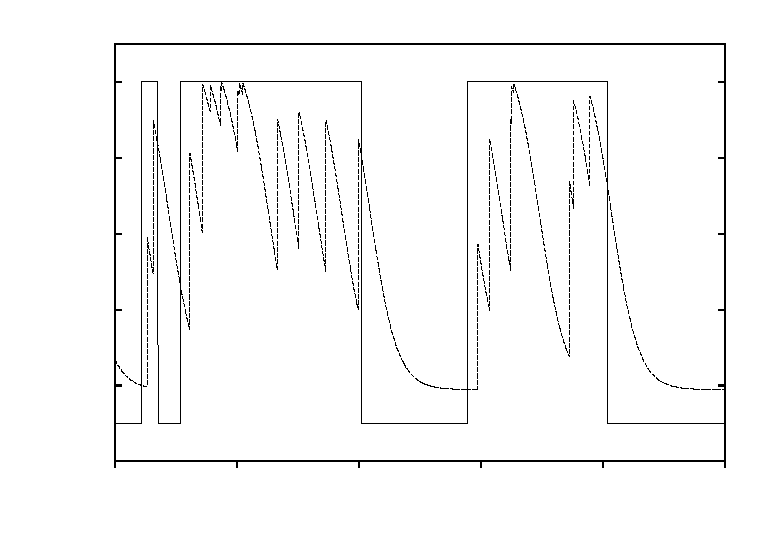
\includegraphics{estrate}}%
    \gplfronttext
  \end{picture}%
\endgroup
}
\end{center}
\end{frame}

\subsection{ISI distribution}
\begin{frame}
\frametitle{Inter-Spike Interval Distribution}
\begin{itemize}
\item The firing rate of neurons in-vivo can only be estimated, not measured directly.
\pause
\item Instead, the \emph{inter-spike interval} (ISI) distribution can be measured.
\end{itemize}
\pause
Given an inhomogeneous Poisson rate $f(t)$, the probability density function (pdf) of the associated ISI distribution can be calculated:
\begin{equation*}
p_{ISI}(t) = f(t) e^{\int_0^t f(s)\, ds}
\end{equation*}
\end{frame}

\begin{frame}
\frametitle{}
With the rate function $r(t)$ as above, get:
\begin{equation}
p_{ISI}(t) = \rho e^{-\alpha t} + (1-\rho)e^{-\beta t}
\end{equation}
\bigskip
This is the pdf of the hyper-exponential distribution $H_2$.
\end{frame}
\section{Testing on data}
\begin{frame}
\frametitle{Zebra Finch Data}
\begin{center}
\begin{tabular}{cr}
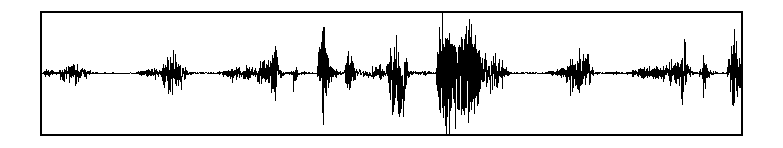
\epsfig{file=images/songwithSpect.eps,width=1.5in} & 20 conspecific songs.\\
{\large $\times 20$}& Each is played ten times.\\
\vdots &\\
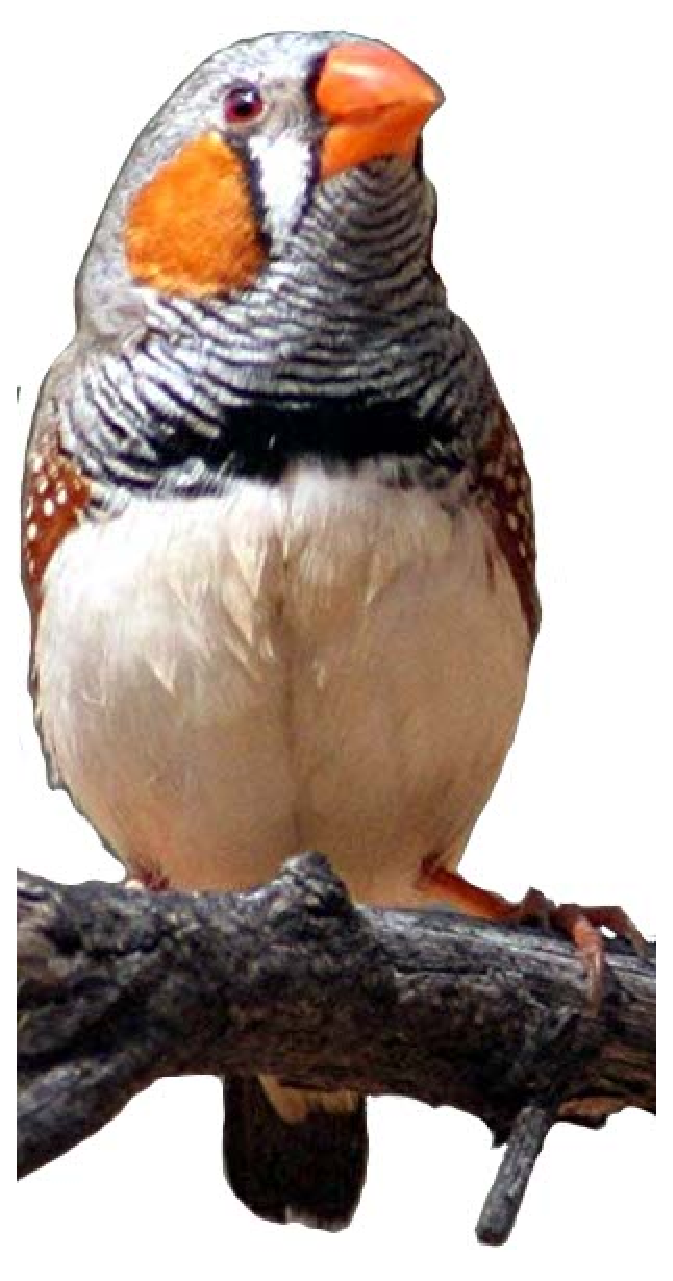
\epsfig{file=images/Finch-Zebra.eps,width=0.25in}& The electrode is in the area L1. \\
\vdots&\\
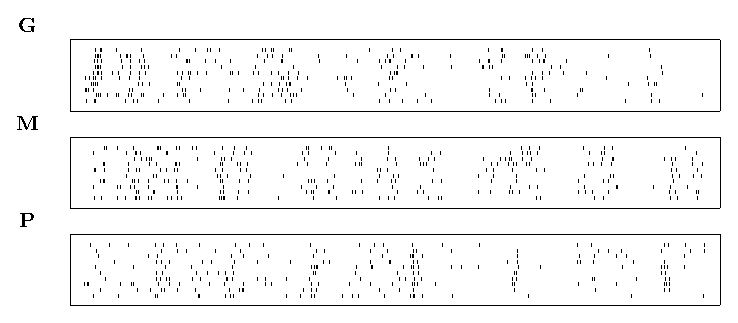
\epsfig{file=images/raster.eps,width=1.5in} & The output is recorded.
 \end{tabular}

\end{center}
\end{frame}

\begin{frame}
\frametitle{Notes on Data}
\begin{itemize}
\item Due to the refractory period, this model will not be observed in a single neuron's response.
\pause
\bigskip
\item Instead, the ten presentations of each stimulus are superimposed to get an \lq{}average response\rq{}.
\pause
\bigskip
\item The data is trained on 16 of the songs and tested on the remaining four songs.
\end{itemize}
\end{frame}

\begin{frame}
\frametitle{Results}
\begin{center}
\resizebox{0.8\textwidth}{!}{% GNUPLOT: LaTeX picture with Postscript
\begingroup
  \makeatletter
  \providecommand\color[2][]{%
    \GenericError{(gnuplot) \space\space\space\@spaces}{%
      Package color not loaded in conjunction with
      terminal option `colourtext'%
    }{See the gnuplot documentation for explanation.%
    }{Either use 'blacktext' in gnuplot or load the package
      color.sty in LaTeX.}%
    \renewcommand\color[2][]{}%
  }%
  \providecommand\includegraphics[2][]{%
    \GenericError{(gnuplot) \space\space\space\@spaces}{%
      Package graphicx or graphics not loaded%
    }{See the gnuplot documentation for explanation.%
    }{The gnuplot epslatex terminal needs graphicx.sty or graphics.sty.}%
    \renewcommand\includegraphics[2][]{}%
  }%
  \providecommand\rotatebox[2]{#2}%
  \@ifundefined{ifGPcolor}{%
    \newif\ifGPcolor
    \GPcolorfalse
  }{}%
  \@ifundefined{ifGPblacktext}{%
    \newif\ifGPblacktext
    \GPblacktexttrue
  }{}%
  % define a \g@addto@macro without @ in the name:
  \let\gplgaddtomacro\g@addto@macro
  % define empty templates for all commands taking text:
  \gdef\gplbacktext{}%
  \gdef\gplfronttext{}%
  \makeatother
  \ifGPblacktext
    % no textcolor at all
    \def\colorrgb#1{}%
    \def\colorgray#1{}%
  \else
    % gray or color?
    \ifGPcolor
      \def\colorrgb#1{\color[rgb]{#1}}%
      \def\colorgray#1{\color[gray]{#1}}%
      \expandafter\def\csname LTw\endcsname{\color{white}}%
      \expandafter\def\csname LTb\endcsname{\color{black}}%
      \expandafter\def\csname LTa\endcsname{\color{black}}%
      \expandafter\def\csname LT0\endcsname{\color[rgb]{1,0,0}}%
      \expandafter\def\csname LT1\endcsname{\color[rgb]{0,1,0}}%
      \expandafter\def\csname LT2\endcsname{\color[rgb]{0,0,1}}%
      \expandafter\def\csname LT3\endcsname{\color[rgb]{1,0,1}}%
      \expandafter\def\csname LT4\endcsname{\color[rgb]{0,1,1}}%
      \expandafter\def\csname LT5\endcsname{\color[rgb]{1,1,0}}%
      \expandafter\def\csname LT6\endcsname{\color[rgb]{0,0,0}}%
      \expandafter\def\csname LT7\endcsname{\color[rgb]{1,0.3,0}}%
      \expandafter\def\csname LT8\endcsname{\color[rgb]{0.5,0.5,0.5}}%
    \else
      % gray
      \def\colorrgb#1{\color{black}}%
      \def\colorgray#1{\color[gray]{#1}}%
      \expandafter\def\csname LTw\endcsname{\color{white}}%
      \expandafter\def\csname LTb\endcsname{\color{black}}%
      \expandafter\def\csname LTa\endcsname{\color{black}}%
      \expandafter\def\csname LT0\endcsname{\color{black}}%
      \expandafter\def\csname LT1\endcsname{\color{black}}%
      \expandafter\def\csname LT2\endcsname{\color{black}}%
      \expandafter\def\csname LT3\endcsname{\color{black}}%
      \expandafter\def\csname LT4\endcsname{\color{black}}%
      \expandafter\def\csname LT5\endcsname{\color{black}}%
      \expandafter\def\csname LT6\endcsname{\color{black}}%
      \expandafter\def\csname LT7\endcsname{\color{black}}%
      \expandafter\def\csname LT8\endcsname{\color{black}}%
    \fi
  \fi
  \setlength{\unitlength}{0.0500bp}%
  \begin{picture}(7200.00,5040.00)%
    \gplgaddtomacro\gplbacktext{%
      \csname LTb\endcsname%
      \put(1078,767){\makebox(0,0)[r]{\strut{} 0}}%
      %\put(1078,1219){\makebox(0,0)[r]{\strut{} 0.02}}%
      \put(1078,1670){\makebox(0,0)[r]{\strut{} 0.04}}%
      %\put(1078,2122){\makebox(0,0)[r]{\strut{} 0.06}}%
      \put(1078,2573){\makebox(0,0)[r]{\strut{} 0.08}}%
      %\put(1078,3025){\makebox(0,0)[r]{\strut{} 0.1}}%
      \put(1078,3476){\makebox(0,0)[r]{\strut{} 0.12}}%
      %\put(1078,3928){\makebox(0,0)[r]{\strut{} 0.14}}%
      \put(1078,4379){\makebox(0,0)[r]{\strut{} 0.16}}%
      \put(2656,484){\makebox(0,0){\strut{} (a)}}%
      \put(4038,484){\makebox(0,0){\strut{} (b)}}%
      \put(5421,484){\makebox(0,0){\strut{} (c)}}%
      \put(176,2573){\makebox(0,0){\strut{}D_n}}%
      \put(4038,154){\makebox(0,0){\strut{}Distributions}}%
      \put(4038,4709){\makebox(0,0){\strut{}Kolmogorov-Smirnov statistics}}%
    }%
    \gplgaddtomacro\gplfronttext{%
    }%
    \gplbacktext
    \put(0,0){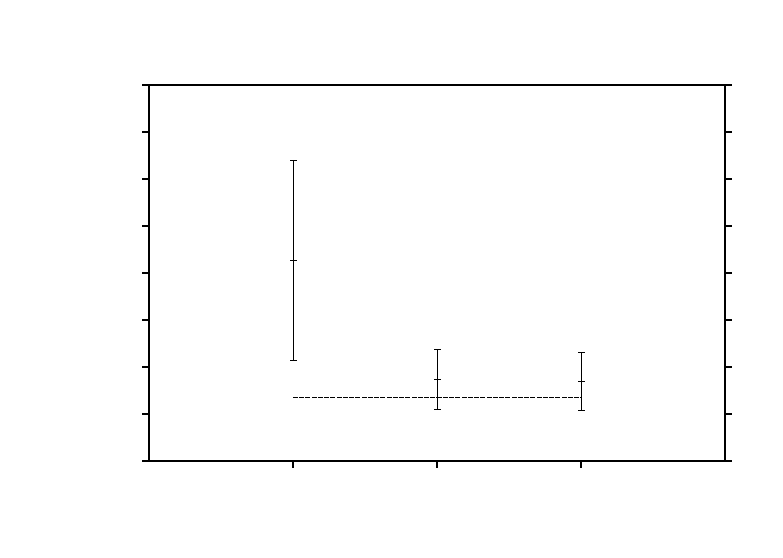
\includegraphics{ksdists}}%
    \gplfronttext
  \end{picture}%
\endgroup
}
\end{center}
\end{frame}

\section{Conclusion}

\begin{frame}
\frametitle{Conclusions}
\begin{itemize}
\item There appears to be evidence of bimodality in the ISI distributions.
\pause
\bigskip
\item This would suggest a bimodality in the firing rate.
\pause
\bigskip
\item Evidence of sparse coding in the auditory forebrain of zebra finches.
\end{itemize}
\end{frame}
\begin{frame}
\frametitle{Thanks}
Special thanks to: \\ \bigskip my supervisor Dr. Conor Houghton, \\ \pause \bigskip the School of Maths here in TCD,\\ \pause \bigskip and the University of Bristol.
\end{frame}
\begin{frame}
\frametitle{Questions?}
\begin{center}
Thank you for listening! \\ \bigskip Any questions?
\end{center}
\end{frame}

\end{document} 